\documentclass[UTF8]{ctexbook}
\usepackage{graphicx}
\usepackage{amsmath}
\title{Latex学习笔记}
\author{张安}
\date{\today}

\bibliographystyle{plain}

\begin{document}
  \maketitle

  \tableofcontents\footnote{“$\backslash$ tableofcontents”命令生成目录}
  \newpage
\chapter{Day1}

\section{数学公式基本方法}

\subsection{行内数学公式}
“\$ \$”包裹的“a\^2+b\^2=c\^2”
\footnote{这里的\^\ 符号不知道为什么没有显示出来}
则会变成行内公式:$a^2+b^2=c^2$
\newline
它会显示在行内,而不是另起一行,通常用于小公式

\subsection{行间的列表公式}
使用如下方法书写行内数学公式 \newline
“$\backslash$begin\{equation\} \newline 公式内容 \newline$\backslash$end\{equation\}”
\newline
该方法可以将公式单独居中输入,如下所示
\begin{equation}
  a(b+c) = ab + ac
\end{equation}
\begin{equation}
  \angle ACB = \pi / 2
\end{equation}
\begin{equation}\label{eq:gougu}
  AB^2 = BC^2 + AC^2
\end{equation}
可以看到,这些公式是自动编号的
\begin{equation}
  \angle ACB = \pi / 2
\end{equation}
\begin{equation}
  AB^2 = BC^2 + AC^2
\end{equation}
并且是全局编号,隔着中间的句子依然是(4),(5)的编号

\section{图表基本表示方法}
使用图表之前,需要添加graphicx包,使用“$\backslash$usepackage\{graphicx\}”命令
\subsection{添加行内图片}
使用“$\backslash$includegraphics$[$width=3cm$]$\{./Figures/Chapter1/Figure1.png\}”命令显示png图片,该图片存放在文档目录的相对路径下
例如: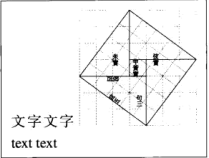
\includegraphics[width=3cm]{./Figures/Chapter1/Figure1.png}

\subsection{添加行间图片}
使用如下图中的方式添加行间图片
\begin{figure}[ht]
  \centering
  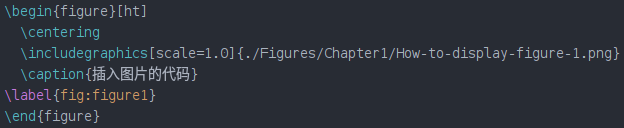
\includegraphics[scale=0.8]{./Figures/Chapter1/How-to-display-figure-1.png}
  \caption{插入图片的代码}
\label{fig:figure1}
\end{figure}
\\
其中,$(1)$使用了figure环境,figure环境包括了可选参数h和t,表明\emph{浮动体可以出现在环境周围文本所在处(here)和一页的顶部(top)}
$(2)$第2行表示后面内容居中$(3)$第3行插入图,scale表示大小.$(4)$caption命令产生自动编号和标题,而lable命令则给图一个标签用以引用。
\newpage
\subsection{添加表格}
通过如下命令来制作一个\textbf{表格}\newline
\begin{figure}[ht]
  \centering
  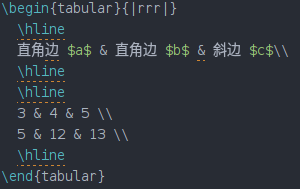
\includegraphics[scale=0.8]{./Figures/Chapter1/How-to-display-table-1.png}
  \caption{显示表格的代码}
\label{fig:table1}
\end{figure}
\newline
\begin{tabular}{|ccc|}
  \centering
  \hline
  直角边 $a$ & 直角边 $b$ & 斜边 $c$\\
  \hline
  3 & 4 & 5 \\
  5 & 12 & 13 \\
  \hline

\end{tabular}

\section{引用以及参考文献}
使用ref,cite,nocite命令进行引用
\\
注意,在使用eqref命令引用公式前,需要在导言区添加''$\backslash$usepackage\{amsmath\}''

\chapter{文字、符号、段落、文本环境}
\section{斜体、粗体}

使用\emph{emph}做出\emph{斜体},使用\textbf{textbf}做出\textbf{粗体}\\
\newcommand\Emph{\textbf}
我们也可以使用newcommand命令定义新的粗体命令“$\backslash newcommand\backslash Emph\{\backslash textbf\}$”,自此以后,我们便可以使用Emph为\Emph{粗体}\\

\section{字号与行距}

\section{编号,项目点}
\textbf{Latex提供了3种列表环境:}
\begin{enumerate}
  \centering
  \item 编号的enumerate环境
  \item 不编号的itemize环境
  \item 使用关键字的description环境
\end{enumerate}
\textbf{列表环境可以多级嵌套:}
\begin{enumerate}
  \item 中文
  \begin{enumerate}
    \item 古代汉语
    \item 现代汉语
    \begin{enumerate}
      \item 普通话
      \item 方言
    \end{enumerate}
    \item 书面语
  \end{enumerate}
  \item English
\end{enumerate}
\textbf{可以用item的参数自行规定enumerate或itemize的编号或是标识符号:}
\begin{enumerate}
  \centering
  \item 带编号的enumerate
  \item[number-one]设置编号为”number-one”
  \begin{itemize}
    \centering
    \item 项目符号的itemize
    \item[\dag] 用$[\backslash dag]$显示十字符号
  \end{itemize}
\end{enumerate}

\section{定理类环境}

\end{document}
